\documentclass[12pt]{article}

\usepackage{amsmath}    % need for subequations
\usepackage{graphicx}   % need for figures
\usepackage{verbatim}   % useful for program listings
\usepackage{color}      % use if color is used in text
\usepackage{subfigure}  % use for side-by-side figures
\usepackage{hyperref}   % use for hypertext links, including those to external documents and URLs

% don't need the following. simply use defaults
\setlength{\baselineskip}{16.0pt}    % 16 pt usual spacing between lines

\setlength{\parskip}{3pt plus 2pt}
\setlength{\parindent}{20pt}
\setlength{\oddsidemargin}{0.5cm}
\setlength{\evensidemargin}{0.5cm}
\setlength{\marginparsep}{0.75cm}
\setlength{\marginparwidth}{2.5cm}
\setlength{\marginparpush}{1.0cm}
\setlength{\textwidth}{150mm}

\begin{comment}
\pagestyle{empty} % use if page numbers not wanted
\end{comment}

% above is the preamble

\begin{document}

\begin{center}
{\large Introduction to \LaTeX} \\ % \\ = new line
\copyright 2006 by Harvey Gould \\
December 5, 2006
\end{center}

\section{Introduction}
\TeX\ looks more difficult than it is. It is
almost as easy as $\pi$. See how easy it is to make special
symbols such as $\alpha$,
$\beta$, $\gamma$,
$\delta$, $\sin x$, $\hbar$, $\lambda$, $\ldots$ We also can make
subscripts
$A_{x}$, $A_{xy}$ and superscripts, $e^x$, $e^{x^2}$, and
$e^{a^b}$. We will use \LaTeX, which is based on \TeX\ and has
many higher-level commands (macros) for formatting, making
tables, etc. More information can be found in Ref.~\cite{latex}.

We just made a new paragraph. Extra lines and spaces make no
difference. Note that all formulas are enclosed by
\$ and occur in \textit{math mode}.

The default font is Computer Modern. It includes \textit{italics},
\textbf{boldface},
\textsl{slanted}, and \texttt{monospaced} fonts.

\section{Equations}
Let us see how easy it is to write equations.
\begin{equation}
\Delta =\sum_{i=1}^N w_i (x_i - \bar{x})^2 .
\end{equation}
It is a good idea to number equations, but we can have a
equation without a number by writing
\begin{equation}
P(x) = \frac{x - a}{b - a} , \nonumber
\end{equation}
and
\begin{equation}
g = \frac{1}{2} \sqrt{2\pi} . \nonumber
\end{equation}

We can give an equation a label so that we can refer to it later.
\begin{equation}
\label{eq:ising}
E = -J \sum_{i=1}^N s_i s_{i+1} ,
\end{equation}
Equation~\eqref{eq:ising} expresses the energy of a configuration
of spins in the Ising model.\footnote{It is necessary to process (typeset) a
file twice to get the counters correct.}

We can define our own macros to save typing. For example, suppose
that we introduce the macros:
\begin{verbatim}
 \newcommand{\lb}{{\langle}}
 \newcommand{\rb}{{\rangle}}
\end{verbatim}
\newcommand{\lb}{{\langle}}
\newcommand{\rb}{{\rangle}}
Then we can write the average value of $x$ as
\begin{verbatim}
\begin{equation}
\lb x \rb = 3
\end{equation}
\end{verbatim}
The result is
\begin{equation}
\lb x \rb = 3 .
\end{equation}

Examples of more complicated equations:
\begin{equation}
I = \! \int_{-\infty}^\infty f(x)\,dx \label{eq:fine}.
\end{equation}
We can do some fine tuning by adding small amounts of horizontal
spacing:
\begin{verbatim}
 \, small space       \! negative space
\end{verbatim}
as is done in Eq.~\eqref{eq:fine}.

We also can align several equations:
\begin{align}
a & = b \\
c &= d ,
\end{align}
or number them as subequations:
\begin{subequations}
\begin{align}
a & = b \\
c &= d .
\end{align}
\end{subequations}

We can also have different cases:
\begin{equation}
\label{eq:mdiv}
m(T) =
\begin{cases}
0 & \text{$T > T_c$} \\
\bigl(1 - [\sinh 2 \beta J]^{-4} \bigr)^{\! 1/8} & \text{$T < T_c$}
\end{cases}
\end{equation}
write matrices
\begin{align}
\textbf{T} &=
\begin{pmatrix}
T_{++} \hfill & T_{+-} \\
T_{-+} & T_{--} \hfill 
\end{pmatrix} , \nonumber \\
& =
\begin{pmatrix}
e^{\beta (J + B)} \hfill & e^{-\beta J} \hfill \\
e^{-\beta J} \hfill & e^{\beta (J - B)} \hfill
\end{pmatrix}.
\end{align}
and 
\newcommand{\rv}{\textbf{r}}
\begin{equation}
\sum_i \vec A \cdot \vec B = -P\!\int\! \rv \cdot
\hat{\mathbf{n}}\, dA = P\!\int \! {\vec \nabla} \cdot \rv\, dV.
\end{equation}

\section{Tables}
Tables are a little more difficult. TeX
automatically calculates the width of the columns.

\begin{table}[h]
\begin{center}
\begin{tabular}{|l|l|r|l|}
\hline
lattice & $d$ & $q$ & $T_{\rm mf}/T_c$ \\
\hline
square & 2 & 4 & 1.763 \\
\hline
triangular & 2 & 6 & 1.648 \\
\hline
diamond & 3 & 4 & 1.479 \\
\hline
simple cubic & 3 & 6 & 1.330 \\
\hline
bcc & 3 & 8 & 1.260 \\
\hline
fcc & 3 & 12 & 1.225 \\
\hline
\end{tabular}
\caption{\label{tab:5/tc}Comparison of the mean-field predictions
for the critical temperature of the Ising model with exact results
and the best known estimates for different spatial dimensions $d$
and lattice symmetries.}
\end{center}
\end{table}

\section{Lists}

Some example of formatted lists include the
following:

\begin{enumerate}

\item bread

\item cheese

\end{enumerate}

\begin{itemize}

\item Tom

\item Dick

\end{itemize}

\section{Figures}

We can make figures bigger or smaller by scaling them. Figure~\ref{fig:lj}
has been scaled by 60\%.

\begin{figure}[h]
\begin{center}
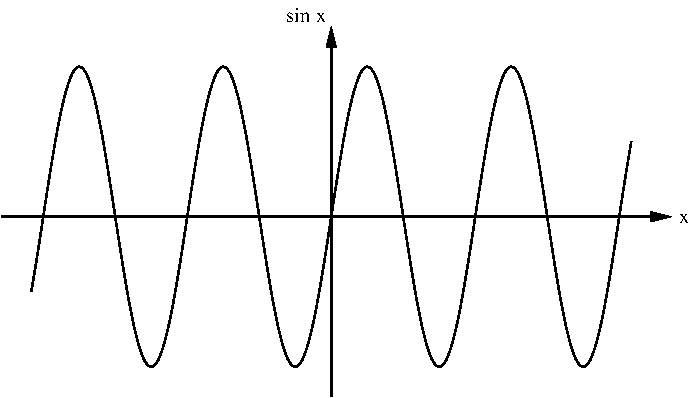
\includegraphics{figures/sine}
\caption{\label{fig:typical}Show me a sine.}
\end{center}
\end{figure}

\begin{figure}[h]
\begin{center}
\scalebox{0.6}{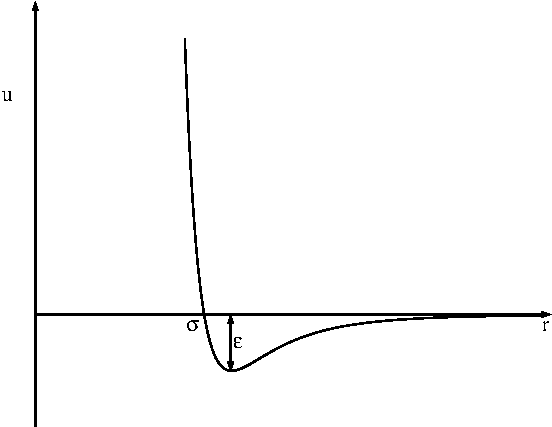
\includegraphics{figures/lj}}
\caption{\label{fig:lj}Plot of the
Lennard-Jones potential
$u(r)$. The potential is characterized by a length
$\sigma$ and an energy
$\epsilon$.}
\end{center}
\end{figure}

\section{Literal text}
It is desirable to print program code exactly as it is typed in a
monospaced font. Use \verb \begin{verbatim} and
\verb \end{verbatim} as in the following example:
\begin{verbatim}
double y0 = 10; // example of declaration and assignment statement
double v0 = 0;  // initial velocity
double t = 0;   // time
double dt = 0.01; // time step
double y = y0;
\end{verbatim}
The command \verb \verbatiminput{programs/Square.java}\ allows
you to list the file \texttt{Square.java} in the directory
programs.

\section{Special Symbols}

\subsection{Common Greek letters}

These commands may be used only in math mode. Only the most common
letters are included here.

$\alpha, 
\beta, \gamma, \Gamma,
\delta,\Delta,
\epsilon, \zeta, \eta, \theta, \Theta, \kappa,
\lambda, \Lambda, \mu, \nu,
\xi, \Xi,
\pi, \Pi,
\rho,
\sigma, 
\tau,
\phi, \Phi,
\chi,
\psi, \Psi,
\omega, \Omega$

\subsection{Special symbols}

The derivative is defined as
\begin{equation}
\frac{dy}{dx} = \lim_{\Delta x \to 0} \frac{\Delta y}
{\Delta x}
\end{equation}
\begin{equation}
f(x) \to y \quad \mbox{as} \quad x \to
x_{0}
\end{equation}
\begin{equation}
f(x) \mathop {\longrightarrow}
\limits_{x \to x_0} y
\end{equation}

\noindent Order of magnitude:
\begin{equation}
\log_{10}f \simeq n
\end{equation}
\begin{equation}
f(x)\sim 10^{n}
\end{equation}
Approximate equality:
\begin{equation}
f(x)\simeq g(x)
\end{equation}
\LaTeX\ is simple if we keep everything in proportion:
\begin{equation}
f(x) \propto x^3 .
\end{equation}

Finally we can skip some space by using commands such as
\begin{verbatim}
\bigskip    \medskip    \smallskip    \vspace{1pc}
\end{verbatim}
The space can be negative.

\section{\color{red}Use of Color}

{\color{blue}{We can change colors for emphasis}},
{\color{green}{but}} {\color{cyan}{who is going pay for the ink?}}

\section{\label{morefig}Subfigures}

As soon as many students start becoming comfortable using \LaTeX, they want
to use some of its advanced features. So we now show how to place two
figures side by side.

\begin{figure}[h!]
\begin{center}
\subfigure[Real and imaginary.]{
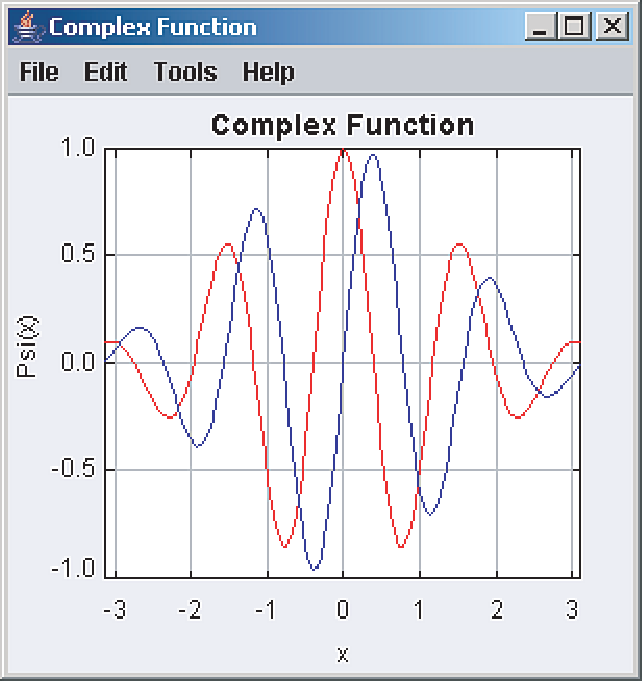
\includegraphics[scale=0.5]{figures/reim}}
\subfigure[Amplitude and phase.]{
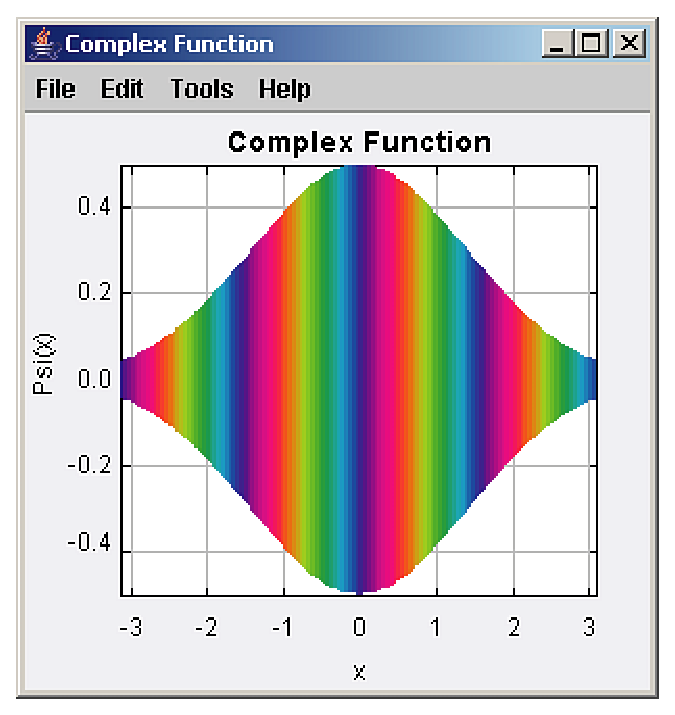
\includegraphics[scale=0.5]{figures/phase}}
\caption{\label{fig:qm/complexfunctions} Two representations of complex
wave functions.}
\end{center}
\end{figure}

We first have to include the necessary package,
\verb+\usepackage{subfigure}+, which has to go in the preamble (before
\verb+\begin{document}+). It sometimes can be difficult to place a figure in
the desired place.

Your LaTeX document can be easily modified to make a poster or a screen
presentation similar to (and better than) PowerPoint. Conversion to HTML is
straightforward. Comments on this tutorial are appreciated.

\begin{thebibliography}{5}

\bibitem{latex}Helmut Kopka and Patrick W. Daly, \textsl{A Guide to
\LaTeX: Document Preparation for Beginners and Advanced Users},
fourth edition, Addison-Wesley (2004).

\bibitem{website}Some useful links are
given at \url{}.

\end{thebibliography}

{\small \noindent Updated 5 December 2006.}
\end{document}
